\chapter{Theoretical background}

\section{Need for new technologies to reduce reliance on fossil-based resources} 
% Lisaksin teoreetilise osa esimeseks peatükiks üldise kirjelduse vajadusest vähendada fossiilsete materjalide osakaalu ning selle mitigeerimiseks 
% on ühe võimalusena võimalik kasutada biotehnoloogilisi protsesse, mis suudavad konverteerida jääk-biomassi erinevateks kemikaalideks ning materjalideks. 
% Siit saaks siis otse edasi liikuda R. toroloidese kirjeldusele, kui ühele potentsiaalsele rakuvabrikule biotehnoloogiliste protsesside läbiviimisel. % Petri soovitus

% Due to the massive increase in the utilization of petroleum, it has 
% been predicted that the world will run short of petroleum by the year 
% 2070 \cite{ShieldsMenard2018}. 

% Besides, its widespread usage has also brought global warming 
% and health concerns due to the release of greenhouse and toxic gases 
% such as carbon monoxide, carbon dioxide, methane, and chlorofluorocarbons. Therefore, alternative energy sources that are easily accessible, 
% greener, and readily available are highly required. Due to properties 
% such as non-toxic, biodegradability, being sulfur-free, and the ability of 
% production from renewable sources, biofuels have gained the interest as 
% an alternative to petroleum. \cite{Saini2020}

Many countries globally are developing a bio-based economy to fight climate change and to lower the
reliance on fossil-based resources \cite{Zuiderveen2023}. In Europe, 
the Bio-Economy Strategy was developed to steer Europe towards a sustainable 
bio-based economy and it was reinforced in the European Green Deal aiming for 
climate neutrality by 2050 \cite{Research2018}. Bio-based products may enhance environmental 
sustainability compared to fossil based equivalents \cite{Zuiderveen2023}.

The shift towards a bioeconomy needs novel processes for production of chemicals, materials, 
and liquid fuels from sustainable substrates, that offer improved life cycle 
assessments, and use less energy to produce. Advancements have highlighted the 
potential of chemicals derived from plant oils as alternative 
feedstocks to the petrochemical industry \cite{Durrett2008}.
Biodiesel is synthesized through the 
transesterification of triacylglycerols with short-chain alcohols 
(primarily methanol or ethanol) to yield monoalkyl esters, specifically fatty acid methyl esters (FAMEs) 
and fatty acid ethyl esters (FAEEs) \cite{Koutinas2014}.

% These bioproducts comprise a broad spectrum of molecules that can be utilized in 
% various applications such as biofuels, cosmetics, plastics, 
% surface coatings, surfactants, lubricants, paints, etc. \cite{Lopes2020}. Bad citation

The demand for vegetable oils has increased rapidly due to the expansion
of the demand for edible oils in the food market (representing over 80\%).
The increasing demand in biodiesel sector also represents an increasing part in the growth of the demand of vegetable oils. \cite{rosillo2009global}
But the production of biodiesel from oilseeds and waste oils does not sustain the 
global demand \cite{Koutinas2014} and food crisis has shown the 
need for the development of second-generation biofuels derived from non-edible sources, 
such as lignocellulosic raw materials and industrial waste streams \cite{Koutinas2011}.

Another promising source of fatty acids for oleochemical production are microbial oils, also called single-cell oils (SCOs), that represent
the triacylglycerides produced by microorganisms \cite{Adrio2017}.
Research has focused on the development 
of biodiesel production from SCOs that are produced via cultivation using oleaginous microorganisms (microorganisms 
capable of accumulating lipids at more than 20\% of the total cellular dry weight (DW)). Biodiesel production from SCOs relies on the utilization of low-value waste streams or residues, thus presenting a sustainable alternative for biofuel production. Moreover, the production of SCOs does not require land or other resources that are typically used for food production and it is not influenced by season or climate. \cite{Koutinas2014} 

\section{\textit{Rhodotorula toruloides}} % {Physiological characteristics} % General Physiological characteristics {Central carbon metabolism}

\textit{Rhodotorula toruloides} (previously \textit{Rhodosporidium toruloides}) is a non-conventional, oleaginous yeast,
which can accumulate lipids up to 76.1\% of cell dry weight \cite{Li2007}. 
What is more, \textit{R. toruloides} has good tolerance to inhibitory compounds that are naturally found in biomass hydrolysates \cite{Hu2009, Bonturi2017}.
\textit{Rhodotorula toruloides} is an exceptional microbial lipid producer and has recently emerged as one of the most promising yeasts for bioproduction \cite{Wu2023, Park2018}.

\textit{R. toruloides} occurs naturally in leaves, soil, sea water, etc. It has a broad substrate range, which has made this yeast popular for producing biological oils from inedible substrates such as pentose sugars and crude glycerol. The majority of the lipids produced by \textit{Rhodotorula toruloides} are triacylglycerol (TAG) contained long-chain fatty acids (C16:0 (palmitic acid), C16:1 (palmitoleic acid), C18:0 (stearic acid), C18:1(oleic acid), and C18:2 (linoleic acid)) and they
are comparable to vegetable oils \cite{Li2007, Vasconcelos2019}.
\textit{R. toruloides} lipid fraction contains also carotenoid pigments, 
omega-3 linolenic acid and heptadecenoic acid,
which makes it a promising organism for production of pharma- and nutraceuticals \cite{Buzzini2007}. 

Fatty acids mainly accumulate as TAGs, and they are produced via four cyclic enzymatic reactions that require 1 adenosine triphosphate (ATP) and 2 nicotinamide adenine dinucleotide phosphate (NADPH) molecules for adding 1 acetyl-coenzyme A (acetyl-CoA) to the fatty acid chain \cite{Lian2015}. During fatty acid synthesis and elongation, acetyl-CoA is the donor of C2-carbon. NADPH is required for reduction steps and it is known to be mainly produced by malic enzyme (decarboxylating malate dehydrogenase, ME), and by glucose 6-phosphate dehydrogenase and phosphogluconate dehydrogenase in the pentose phosphate pathway (PPP). \cite{Tehlivets2007}

Metabolic pathways producing acetyl-CoA and a cofactor NADPH have been subject to metabolic studies in \textit{R. toruloides}. Compared to \textit{Saccharomyces cerevisiae}, \textit{R. toruloides} has several different enzymatic pathways that facilitate the generation of lipid precursors. Important difference is that \textit{R. toruloides} possesses the enzyme ATP-citrate lyase (ACL), which synthesises acetyl-CoA from citrate. ACL has been demonstrated to be upregulated in \textit{R. toruloides} during lipid accumulation \cite{Zhu2012} and it has been suggested to be the main source of acetyl-CoA for lipid synthesis in oleaginous species \cite{Vorapreeda2012}. It has been found that \textit{R. toruloides} also possesses the enzyme phosphoketolase \cite{Tiukova2019a}, which is able to convert fructose-6-phosphate and/or xylulose-5-phosphate into acetyl-phosphate + erythrose-4-phosphate and/or acetyl-phosphate + glyceraldehyde-3-phosphate \cite{Evans1984}, producing an acetyl residue (acetyl-phosphate) directly from a C5-substrate. Thus, phosphoketolase is a more efficient way of providing acetyl-CoA compared to the decarboxylation of pyruvate to acetyl-CoA, where one third of the carbon substrate is lost \cite{Tiukova2019a}.
But the upregulation of phosphoketolase during nutrient limitation in \textit{R. toruloides} has not been acknowledged \cite{Tiukova2019a}.

It has been found that in oleaginous yeast malic enzyme is an important enzyme involved in the production of NADPH \cite{Ratledge2002}, but the role of ME in \textit{R. toruloides} is not clearly understood. Proteomics analysis of \textit{R. toruloides} has suggested that NADPH is mainly produced through the pentose phosphate pathway (when grown on xylose and glucose) \cite{Zhu2012}. Lipid biosynthetic reactions downstream of acetyl-CoA synthesis do not significantly differ between oleaginous and non-oleaginous yeast species \cite{Fakas2016}. %\cite{Tiukova2019}

\section{Overview of growth laws in oleaginous microorganisms}

It has been well-established that an imbalance of nutrients in the culture medium triggers lipid accumulation in oleaginous microorganisms. When a crucial nutrient, typically nitrogen, is depleted, cells continue to assimilate excess carbon substrate and transform it into storage fat. \cite{Ratledge2002} Thus, the carbon-to-nitrogen ratio (C/N) is a significant factor in initiating lipid accumulation \cite{Lopes2020}.
The cells take in carbon faster than they can convert it into new cells, so the surplus carbon is stored by turning it into lipid. This lipid accumulation necessitates a slower cell growth rate, allowing the excess carbon to be assimilated more quickly than it can be converted into biomass, thus directing the surplus carbon into lipid. This process of lipid accumulation can also be accomplished in continuous culture with oleaginous yeast, where it is essential to maintain a sufficiently 
low dilution rate (growth rate) to enable the cells to assimilate the glucose. Continuous cultivation studies have clearly demonstrated that the lipid synthesis rate is slower than the maximum growth rate. \cite{Ratledge2002}

The first major biochemical distinction identified between oleaginous and non-oleaginous yeast species was the presence of ATP-citrate lyase in oleaginous yeast during lipid accumulation. This enzyme has been shown to be crucial for a eukaryotic microbial cell to accumulate significant amounts of triacylglycerol lipids. Yeasts without ACL 
invariably had low lipid cell contents. However, some yeasts that had ACL activity did not accumulate lipids, suggesting that some other enzyme activities are also necessary for lipid accumulation. \cite{Ratledge2002}

It has been found that another important enzyme in lipogenesis is malic enzyme, which generates NADPH used by fatty acid synthase (FAS). 
NADPH is also generated by glucose-6-phosphate dehydrogenase, hosphogluconate dehydrogenase, and NADP-dependent isocitrate dehydrogenase. When malic enzyme activity was inhibited using selective inhibitors (sesamol), lipid content in the cells decreased by almost 90\% (from 24\% of the cell biomass to 2\%), without significantly 
affecting growth. This led to the conclusion that sesamol was specifically inhibiting both the cytoplasmic and membrane-bound malic enzymes, and without malic enzyme, the cell was unable to accumulate lipid or carry out its desaturations. \cite{Ratledge2002}

Wynn and Ratledge (1997) further demonstrated that in a mutant of \textit{Aspergillus Nidulans} that lacked malic enzyme activity, only half the lipid that had been previously produced by a competent strain under nitrogen-limited growth conditions, was now produced. Fatty acid biosynthesis itself was still functional, and phospholipids were 
produced. Meaning that the cells can function without malic enzyme, but they cannot produce storage triacylglycerols in any significant quantity - without malic enzyme activity, the flow of carbon from glucose to lipid was significantly reduced, and only essential lipids were produced, presumably using other sources of NADPH. \cite{Ratledge2002}

\section{Overview of microbial cultivation methods}

% Here you have to explain that in biotechnology, especially with industrial applications like R. toruloides, microbes are 
% grown in bioreactors from small to large scale. What parameters are controlled in cultivations. Don’t be afraid to cite old books 
% or papers that you can find. Please, explain batch, fed-batch and steady-state cultivations. Steady state is what is being simulated 
% by GEMs. While sometimes, batch growth is assumed to represent a steady state during the time when cells grow exponentially:)

% Also, please check what experiments have been carried out in those publications of R. toruloides that you have cited throughout 
% this work - you will see batch growth, turbidostat, maybe fed-batch. Pay attention to Shen et al. 2013 and 2017 where steady state 
% cultivation was done. They focused on biomass analyses, but don’t have glucose rates. That’s why we use our latest lab data.

Microorganisms play a crucial role in biotechnology, being utilized for the production of a variety of bioproducts. In an industrial setting, microbes are cultivated in large-scale bioreactors to manufacture biopharmaceuticals, dietary supplements, biofuels, or other chemical substances. The cultivation process requires careful control of various parameters to ensure optimal growth conditions for the microbes. These parameters include temperature, pH, oxygen levels, agitation (stirring), and pressure. It is vital to regulate these factors to provide a suitable physical and chemical environment for the cells, thereby enhancing their productivity. There are three main methods for microbial cultivation: batch, fed-batch and steady-state. \cite{YangSha2019}

In a batch culture, no nutrients are added or waste removed. Microorganisms growing in such a closed culture follow a pattern known as the growth curve, which, when plotted against time, reveals different phases. The first phase of the growth curve, the lag phase, represents a small number of cells (known as an inoculum) introduced into a fresh culture medium, a nutrient-rich broth that promotes growth. During this phase, the cell count remains unchanged, but the cells increase in size and are metabolically active, producing proteins necessary for growth. The log phase follows next, where the cells divide actively, and their count increases exponentially. Cells in the log phase exhibit a constant growth rate and uniform metabolic activity, making them ideal for industrial applications and research work. \cite{2024Microbial}

However, as the cell count rises during the log phase, several factors contribute to a slowdown in the growth rate. Accumulation of waste products, gradual depletion of nutrients, and limited oxygen availability due to increased consumption all contribute to this slowdown. This leads to a plateau in the total number of live cells, known as the stationary phase. In this phase, the number of new cells created by cell division equals the number of cells dying, resulting in a relatively stagnant total population of living cells. As the culture medium becomes saturated with toxic waste and nutrients get exhausted, cell death outpaces cell division, leading to an exponential decrease in the cell count. This phase is named the death or decline phase. \cite{2024Microbial}

Fed-batch cultivation is a variation of batch cultivation. Microorganisms are initially grown under batch conditions, after which nutrients are incrementally added to the fermenter throughout the remaining cultivation duration. The addition of fresh nutrients typically results in significant biomass accumulation during the exponential growth phase. Therefore, fed-batch cultivation is particularly useful for bioprocesses aiming for high biomass density or high product yield when the desired product is positively correlated with microbial growth. \cite{YangSha2019}

In industrial applications and research work, it is beneficial to keep cells in the logarithmic phase of growth.
A steady-state cultivation, also called chemostat, enables the maintainance of a continuous 
culture thanks to the addition and removal of fluids, adjusted to keep the culture in the logarithmic phase of growth. \cite{2024Microbial} Fresh medium is continuously added to the fermenter, while used medium, (toxic) metabolites and cells are simultaneously harvested. Unlike fed-batch cultivation, the maximum working volume of the vessel does not limit the amount of fresh medium or feed solution that can be added to the culture during the process. When the addition and removal rates are equal, the culture volume remains constant. The cellular growth rate and environmental conditions, like the concentrations of metabolites, remain constant. Steady-state cultures can last for days, weeks, or even months, significantly reducing downtime and making the process more economically competitive. \cite{YangSha2019}

Metabolic analysis requires experimental data for the 
determination of metabolic fluxes. These flux calculations 
are based on the measurements of specific rates for the uptake of substrate and the formation of product during cultivations.
The specific substrate uptake rate, denoted as $r_s$ (expressed in grams or moles of the compound per gram or mole of biomass and unit time), represents the rate at which cells take up a substrate (the flux into the cells). In steady-state cultivations, this rate can be calculated as the difference between the glucose concentration in the feed and that in the bioreactor, multiplied by the dilution rate. The specific product formation rate $r_p$ represents the fluxes of metabolic products out of the cell, that is, the rate at which products are secreted. Additionally, there is an accumulation of biomass within the cell and that rate is represented as a flux of the specific growth rate, $\mu$ expressed in \unit{1/h}, that equals the dilution rate in a steady-state chemostat. \cite{Stephanopoulos1998}


% A study attempting to establish optimal production conditions, found that the lipid yield of oleaginous yeasts was greatly 
% improved by using the continuous culture mode, indicating that it is superior to 
% the batch culture mode for lipid production. \cite{Ghazani2022}

% The density of the culture is defined as the number of cells per volume. \cite{2024Microbial}


\section{Genome-scale metabolic modeling} %incl. Constraint-based modeling, kinetic modeling, steady-state, limitations, e.g. regulation

Cellular metabolism involves numerous reactions that are part of the conversion of resources into energy and precursors needed for 
biosynthesis. Rates of these reactions are called fluxes and they illustrate metabolic activity. Flux of a reaction results from a combined regulation of many biological levels (transcription, translation, post-translational modifications and protein-protein interactions). \cite{Nidelet2016} Hence, metabolic fluxes represent cellular phenotype under certain conditions and therefore analyzing the flux distribution of metabolites is very useful for studying cell metabolism \cite{Nielsen2003}. It is difficult to measure intracellular fluxes experimentally, but it is possible to predict these fluxes thanks to metabolic models \cite{Nidelet2016}.

When the first full genome sequences were published in the 1990s, in principle it became possible to identify all the gene products involved in a given organism's biological processes. This, with well studied biochemistry of metabolism, allowed the reconstruction of metabolic networks on a genome-scale for a target organism. Such reconstructions, containing biochemical, genetic, and genomic (BiGG) knowledge, can be converted into a mathematical format allowing the formulation of genome-scale models (GEMs). \cite{Palsson2009} Thanks to the fact that GEMs account for all known genes, proteins, and biochemical reactions, it is possible to conduct systematic analysis of a given organism's metabolism, where typically the objective is to obtain an overview of possible flux patterns. %Genome-scale metabolic models simulate steady state.
It is possible to integrate omics data and experimental metabolic fluxes to GEMs for generating a holistic view of metabolism in different physiological states, enabling a greater understanding of cellular physiology, providing valuable information for metabolic engineering to develop better microbial factories \cite{Kerkhoven2022}. 

The metabolic reconstruction process usually is very labor- and time consuming. For well-studied, medium genome sized bacteria it can take around six months to reconstruct the model. 
The metabolic reconstruction of human metabolism can take up to two years for six people. The reconstruction process is often iterative, for example, the reconstruction of metabolic 
network of \textit{Escherichia coli} has been expanded and refined throughout the last 19 years. Despite growing experience and 
knowledge, it is still not possible to completely automatically reconstruct high-quality metabolic networks which can be used as reliable predictive models. \cite{Thiele2010} 

\subsection{Constraint-based modeling}

Genome-scale metabolic models (GEMs) are commonly used to compute metabolic phenotypes. However, these models also depend on a set of constraints due to various factors that limit cellular functions. These constraints fall into four categories: basic physico-chemical constraints, spatial or topological constraints, condition-dependent environmental constraints, and self-imposed or regulatory constraints. \cite{Price2004}

Physico-chemical constraints are fundamental and provide inviolable constraints on cell functions, including the conservation of mass, energy, and momentum. Topobiological constraints arise from the crowding of molecules inside cells, affecting the form and function of biological systems. For instance, bacterial DNA, which is about 1,000 times longer than a cell, must be tightly packed yet easily accessible for transcription. \cite{Price2004}
Environmental constraints, which are time and condition dependent, include factors like nutrient availability, pH, temperature, osmolarity, and the availability of electron acceptors. These constraints are crucial for the quantitative analysis of microorganisms and require defined media and well-documented environmental conditions for integrating data into accurate and predictive quantitative models. Regulatory constraints are self-imposed and subject to evolutionary change, allowing the cell to eliminate suboptimal phenotypic states. These constraints are implemented in various ways, including the amount of gene products made and their activity. \cite{Price2004}

A significant limitation of conventional GEMs is that they do not account for enzyme abundances and kinetics, which limit metabolic fluxes. These models often assume that the uptake rate of the carbon source limits production, which may oversimplify the situation. \cite{Sanchez2017} The synthesis of enzymes is resource- and energy-intensive, and their catalytic capacities are limited by their kinetics. Furthermore, the quantity of enzymes is space-constrained. \cite{Kerkhoven2022}

An increase in the requirement of an enzyme or a pathway would be a trade-off for other functions. Experimental evidence suggests that resource re-allocation could be an effective strategy in response to nutrient and growth shifts, demonstrating the biological significance of proteome constraints. \cite{Chen2023} Incorporating such constraints into a metabolic model can lead to more realistic results by reducing simulated flux distributions to those that are most economic and limiting the phenotypes that the model can simulate. \cite{Kerkhoven2022}
% Conventional genome-scale metabolic models are constrained by three factors: (1) the stoichiometry of the network; (2) upper and lower limits for specific reactions (e.g. substrate uptake reactions); and (3) the assumption of a steady state. \cite{Kerkhoven2014} 
Overview of a reconstruction of a GEMs is shown in the Figure \ref{GEMs}.
\begin{figure}[H]
    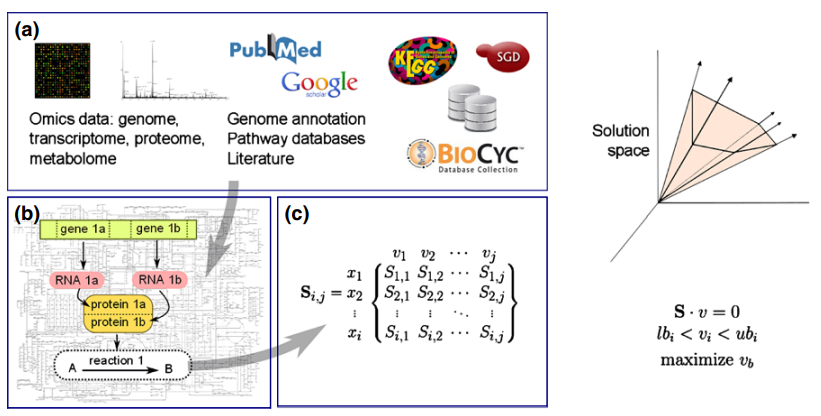
\includegraphics[width=\linewidth]{GEMs.png}
    \caption{Reconstruction of a GEM. (a) The genome annotation is used 
    to reconstruct the draft. (b) Gene-protein-reaction relationships are defined for the metabolic model. 
     (c). A solution space is defined from the constraints applied to the model. Figure is from article \cite{Kerkhoven2014}.}
    \label{GEMs}
\end{figure}

% % Enzyme constrained GEMs - for now these can be excluded

% Integration of enzyme constraints and proteomics data into GEMs was first enabled by the GECKO toolbox \cite{Sanchez2017}, allowing the study of phenotypes constrained by 
% protein limitations. GECKO is a method for enhancement of GEMs with Enzymatic Constraints using 
% Kinetic and Omics data, developed in 2017. This method extends the classical FBA 
% approach by incorporating a detailed description of the enzyme demands for the metabolic reactions in a network, accounting for all types of enzyme-reaction 
% relations, including isoenzymes, promiscuous enzymes and enzymatic complexes. Moreover, GECKO enables direct integration of proteomics abundance data, 
% if available, as constraints for individual protein demands, represented as enzyme usage pseudo-reactions, whilst all the unmeasured enzymes in the network 
% are constrained by a pool of remaining protein mass. \cite{Domenzain2022}

% Every metabolic reaction flux has a
% biological constraint that is equal to the enzyme's concentration multiplied by its turnover number ($k_{cat}$). Enzyme constraint is
% defined as the maximum rate of enzymatic reaction ($v_{max}$) that the metabolic flux cannot exceed. Enzyme-constrained GEMs thereby 
% ensure that each metabolic flux does not exceed its biological maximum capacity, 
% equal to the product of the enzyme's abundance and turnover number. \cite{Sanchez2017}

% Phenomenological constraint is imposed on metabolic flux ($v; mmol/gDCW/h$), formulated as enzyme
% kinetics: $v <=  E \cdot k_{cat}$, where $E$ is protein abundance (mmol/gDCW) and $k_{cat}$ is the enzyme's turnover number (1/s),
% provided with an upper limit on individual or total protein abundances. The integration of
% enzymatic constraints in \textit{S. cerevisiae} has significantly improved phenotype prediction. \cite{Sanchez2017}

\subsection{Flux balance analysis}

% GEMs can simulate metabolic flux distributions by optimization of an objective function that describes the 
% perceived cellular objective that propels 
% metabolism, by flux balance analysis (FBA). \cite{Kerkhoven2022}
Flux balance analysis (FBA) is a mathematical approach for analyzing the flow of metabolites through a metabolic network. It is a commonly employed method for investigating biochemical networks, especially the genome-scale metabolic network reconstructions. Using FBA, it is possible to predict an organism's growth rate or the production rate of a biotechnologically important metabolite. \cite{Orth2010}

The initial phase in FBA involves the mathematical representation of metabolic reactions. The reconstructed genome-scale networks can be transformed into mathematical stoichiometric matrices $\mathbf{S}\in\mathbb{R}^{(m\times n)}$, where each row corresponds to one unique metabolite (for a system with $m$ metabolites) and each column corresponds to an individual reaction ($n$ reactions).
Each column's entries are the stoichiometric coefficients of the metabolites involved in a reaction. A negative coefficient is assigned to each metabolite that is consumed, while a positive coefficient is assigned to each metabolite that is produced. A stoichiometric coefficient of zero is assigned to each metabolite that does not participate in a specific reaction. The stoichiometric matrix $\mathbf{S}$ is sparse, as most biochemical reactions involve only a few different metabolites.
The vector $\mathbf{v}$ represents the fluxes of all the reactions in the network and it has a length of $n$. \cite{Orth2010}

% These stoichiometries impose constraints on the flow of metabolites through the network, defining the solution space of the metabolic network. \cite{Orth2010}

% Other constraints, such as lower and upper bounds for specific reactions, also need to be mathematically described for in silico analysis. Constraints can be classified as either balances or bounds. Balances are associated with conserved quantities and phenomena, such as energy, mass, redox potential and momentum, while bounds limit the numerical ranges of individual variables and parameters (e.g. concentrations, fluxes, kinetic constants). Both types of constraints limit the functional states of reconstructed networks, thereby defining a solution space that represents the phenotypic potential of an organism. \cite{Price2004}

At steady-state, which is simulated by GEMs, there is neither accumulation nor depletion of metabolites in a metabolic network, meaning the rate of production of each metabolite in the network must equal its rate of consumption. 
This flux balance can be mathematically represented as in Equation \eqref{eq:Sv=0} \cite{Price2004}:
\begin{equation}
    \mathbf{S}\cdot \mathbf{v} = \mathbf{0},
    \label{eq:Sv=0}
\end{equation}
where $\mathbf{S}$ is the stoichiometric matrix and $\mathbf{v}$ is the vector of the fluxes.
Any vector $\mathbf{v}$ that satisfies this equation is said to be in the null space of $\mathbf{S}$. In any realistic large-scale metabolic model, there are more reactions than there are compounds ($n > m$). This means that there are more unknown variables than equations, so there is no unique solution to this system of equations. \cite{Orth2010} Thus, the solution space is further constrained by a set of upper and lower bounds on the fluxes: 
\begin{equation}
    a_i < v_i < b_i,
    \label{eq:bounds}
\end{equation}
where $v_i$ is the flux of a certain reaction (usually experimentally measured reactions), and $a_i$ and $b_i$ are the upper and lower bounds of the flux, respectively.
% Without constraints, the flux distribution may lie at any point in a solution space. When mass balance constraints imposed by the stoichiometric matrix $\mathbf{S}$ and capacity constraints imposed by the lower and upper bounds ($a_i$ and $b_i$) are applied to a network, it defines an allowable solution space. The network may acquire any flux distribution within this space, but points outside this space are denied by the constraints. \cite{Orth2010}

The next phase in flux balance analysis involves defining a biological objective that aligns with the research problem being studied. Constraints define a spectrum of potential solutions, but it is still possible to pinpoint and analyze individual solutions within this space. From a mathematical standpoint, the objective is represented by an objective function, which quantifies the contribution of each reaction to the phenotype. For instance, the biomass reaction, which drains precursor metabolites from the system in accordance with their relative stoichiometries, predicts biomass production. The biomass growth rate reaction is then scaled so that its flux matches the organism's exponential growth rate, denoted by $\mu$. \cite{Orth2010}

Another examples of functions used as objective function, are the maximum ATP generation or a specific product formation \cite{Kerkhoven2014}. Also growth-associated maintenance (GAM) and non-growth-associated maintenance (NGAM) reactions can be used. 
GAM and NGAM reactions account for additional energetic requirements in the form of ATP for growth, beyond metabolic costs \cite{Feist2007}.
GAM accounts for the energy needed for cell replication, including macromolecular synthesis (proteins, deoxyribonucleic acid (DNA), and ribonucleic acid (RNA)). Determining GAM is best achieved through chemostat growth experiments. NGAM represents ATP requirements for cell maintenance that is not related to growth (in GEMs it is noted as an ATP hydrolysis reaction). The rate of this reaction can be estimated from growth experiments. \cite{Thiele2010}

FBA uses linear programming to find such vector $\mathbf{v}$ that satisfies constraints mentioned above (Equations \eqref{eq:Sv=0} and \eqref{eq:bounds}) and also maximizes or minimizes the given objective function (see Figure \ref{fig:Solution_space}). \cite{Orth2010}
The COBRA \cite{Becker2007} and RAVEN \cite{EduardKerkhoven2024} toolboxes can be used for solving this kind of optimization problem  for large systems of equations efficiently. Both toolboxes are freely available in Matlab, and the COBRA package is also available in Python. These toolboxes use models that are saved in the Systems Biology Markup Language (SBML) \cite{Hucka2003} format.
\begin{figure}[H]
    \includegraphics[width=\linewidth]{FBA_solution_space.jpg}
    \caption{Conceptual basis of constraint-based modeling and FBA. The figure is from \cite{Orth2010}.}
    \label{fig:Solution_space}
\end{figure}

% FBA is commonly used to assess the biotechnological potential of 
% microorganisms and identify genetic modifications that could enhance the cell performance. Its key applications include:
% (1) instructions for metabolic engineering;
% (2) biological interpretation and discovery through 
% contextualizing high-throughput data;
% (3) creating a computational framework;
% (4) explaining evolutionary aspects;
% (5) describing multispecies communities. \cite{Kerkhoven2014}

% Sampling of the solution space and optimal solution
Flux balance analysis provides only a single optimal solution of the solution space, limiting insight into all of the solution space \cite{Becker2007}. 
An alternative approach to FBA is uniform random sampling of the flux space, which fully determines the range of feasible steady-state fluxes, within the network, given certain physicochemical constraints \cite{Price2004a}.   
This method does not necessitate the definition of an objective function \cite{Bordel2010}. From sampling solutions, the average and standard deviation for each metabolic flux in the GEM can be calculated.
% An alternative approach to FBA involves sampling of the solution space by considering all permissible flux distributions based on mass balance (stoichiometric) and flux capacity constraints. Uniform random sampling of the solution space is a method to understand the permissible metabolic flux space under any environmental condition. 
The flux distributions derived from this sampling can answer questions about the most probable flux value for any reactions and correlations between two reactions under given constraints. \cite{Becker2007}

% \textbf{Limitations of GEMs}

% GEMs and kinetic models both have their advantages
% and drawbacks. GEMs are comprehensive but are dependent on a pseudosteady state and in their current form
% do not take regulation, such as gene-protein and protein-protein level interactions, allosteric regulation or 
% regulation at post-translational level, into account. At the same time, kinetic models require parameter values that are
% difficult to estimate at the global scale. As neither of them can fully replace the other, there has been a considerable
% effort on combining these two approaches in a singular model or applying them in succession. \cite{Kerkhoven2014}

% GEMs in combination with global datasets are invaluable for detecting
% the metabolic bottlenecks, but due to lack of kinetic data about enzyme activities or regulation mechanisms they
% are limited in their predictive power. Applying kinetic models on metabolic bottlenecks previously detected with
% GEMs can help to understand the regulation or kinetics of these specific enzymatic steps, as one would not need
% model parameters for the whole system. \cite{Kerkhoven2014}

\section{Genome-scale metabolic models of \textit{Rhodotorula toruloides}} 
% Tuua välja need erinevad ülegenoomsed mudelid, mis on loodud ning nende peamied iseärasused ja erinevused üksteisest.
% NP11, iRhtoC, IFO0880, IFO0880\_jsb, 

\textbf{rhto-GEM}

The first genome-scale model of \textit{R. toruloides} metabolism named rhto-GEM was presented in 2019 by Tiukova et al. \cite{Tiukova2019}. The model includes 4869 genes, 897 reactions, and 3334 metabolites. This model is based on the genome sequence of \textit{R. toruloides} strain NP11 \cite{Zhu2012} (which is accessible from NCBI database \cite{NP11genome}). For the reconstruction of the metabolism parts that are relatively conserved between fungal species, the well-curated GEM of \textit{Saccharomyces cerevisiae} was utilized as template model (yeast-GEM version 8.2.0, 16). Orthologous genes were identified through bi-directional BLASTP against the \textit{S. cerevisiae} S288c reference genome.

To transform the draft model to the first version of the \textit{R. toruloides} GEM, additional manual curation was performed where remaining template-derived genes were replaced by their \textit{R. toruloides} 
ortholog where possible or otherwise deprecated. The lipid metabolism of \textit{R. toruloides} was described applying the SLIMEr formalism as previously described for \textit{S. cerevisiae}, which allows direct integration of lipid class and acyl chain experimental distribution data \cite{Sanchez2019}. As the acyl chain distribution of \textit{R. toruloides} is different from \textit{S. cerevisiae}, e.g. the presence of C18:2 and C18:3, this required extensive manual curation of the SLIMEr reactions. \textit{R. toruloides} specific reactions and pathways, such as carotene and torulene biosynthesis, synthesis and degradation of C18:2 and C18:3 fatty acids, and mitochondrial beta-oxidation were subsequently manually curated. \cite{Tiukova2019}

The model incorporates knowledge derived from genomics and proteomics data generated for \textit{R. toruloides} and was validated using cultivation data. Simulations of rhto-GEM on various carbon sources showed good match with experimentally reported growth rates. The model analysis helped to identify potential genetic engineering strategies for enhanced lipid production. \cite{Tiukova2019}


\textbf{iRhto1108}

In the same year that Tiukova et al. introduced rhto-GEM, Dinh et al. presented another \textit{R. torluoides} 
genome-scale metabolic model named iRhto1108 \cite{Dinh2019}. This model was built upon functional genomics data from \cite{Coradetti2018} and prior knowledge. The model is based on the metabolic network of the strain IFO0880 \cite{Coradetti2018} (available from JGI database \cite{IFO0880_v4}). It includes 2204 reactions, 1985 metabolites and 1108 genes. 

The authors supplemented and integrated previous knowledge with in-house generated biomass composition and experimental
measurements related to the metabolic capabilities of the organism. 
The iRhto1108 model incorporates yeast biochemistry information from (i) previously constructed genome-scale models (\textit{S. cerevisiae} yeast 7.6 \cite{Aung2013}, (ii) KBase fungal
models \cite{Arkin2018}), and (iii) \textit{R. toruloides} specific information
extracted from the primary literature \cite{Coradetti2018}\cite{Jagtap2017}\cite{Kot2018}. 

% An NGAM value of 1.01 mmol gDW-1 hr-1 for both conditions was recovered. In contrast, the growth associated maintenance
% (GAM) was condition-dependent with a value of 140.98 mmol gDW-1
% under carbon limited and 154.94 mmol gDW-1 under nitrogen limited
% conditions. In yeast 7.6, NGAM is not modeled (though an earlier
% S. cerevisiae model (Mo et al., 2009) reported an NGAM value of 1 mmol
% gDW-1) and the GAM value is 59.28 mmol gDW-1. The GAM value
% quantifies growth-associated energy costs that are not captured in the
% biomass equation, alluding to higher energy demands for R. toruloides
% growth compared to S. cerevisiae. \cite{Dinh2019}

% In rhto-GEM model v. 1.1.1 (Tiukova et al., 2019), a non-condition-specific GAM value of
% 132.7 mmol gDW-1 and NGAM value of 3 mmol gDW-1 hr-1 were reported. These values generally match the iRhto1108’s corresponding
% entries under carbon limitation. \cite{Dinh2019}

% Despite careful curation, a large number of blocked reactions (i.e., 677 out of
% 2204) remained in the model spanning multiple pathways. Most of them
% are transport reactions (i.e., 194 reactions) connecting the network. The
% rest participate in secondary metabolism and degradation of amino acids,
% fatty acids, and lipids. We chose to keep them in the hope that they would
% aid in gap-filling attempts in the future.

The essential metabolic functions and growth capability of the model were thoroughly validated with experimental results, including gene essentiality \cite{Coradetti2018} and growth data. The iRhto1108 model was successful in reproducing the lipid accumulation phenotypes observed in experiments. It can effectively represent the metabolism of \textit{R. toruloides} and provide valuable predictions that have been validated with experimental data, including suggestions for genetic alterations that could lead to triacylglycerol overproducing strains. \cite{Dinh2019} Considering that \textit{R. toruloides} is a non-conventional microorganism, the iRhto1108 model has been a promising start for GEMs of \textit{R. toruloides}, and it holds potential to assist in future research on that yeast. 

Two versions of the model were created, namely iRhtoC and iRhtoN, corresponding to conditions limited by carbon and nitrogen, respectively. These two versions are identical with the exception of the biomass reaction, acyl composition reaction, and the growth associated maintenance reaction. Experimental measurements were conducted to determine the organism-specific macromolecular composition and ATP maintenance requirements under these two separate growth conditions. \cite{Dinh2019}


\textbf{Rt\_IFO0880}

In 2021, a comprehensive multi-omics analysis of lignocellulosic carbon utilization in \textit{R. toruloides} was conducted by Kim et al., leading to the reconstruction of a genome-scale metabolic network named Rt\_IFO0880 \cite{Kim2021}. This metabolic reconstruction consists of 1106 genes, 1934 reactions, and 2010 metabolites across nine compartments.

The initial draft of the metabolic network reconstruction was built using high-quality metabolic network models of model organisms and orthologous protein mapping. The draft was then manually curated into a metabolic model, with the aid of functional annotation and a variety of multi-omics data, including transcriptomics, proteomics, metabolomics, and RB-TDNA sequencing.
The authors identified numerous incorrect reactions, particularly in fatty acid biosynthesis and beta-oxidation. The reactions and genes in the central metabolic pathways were manually verified for their co-factor usage and localization. The biomass reaction was updated using multi-omics and other experimental measurements. Updates included the DNA composition (using the genome sequence), RNA composition (using transcriptomics data), amino acid composition (using proteomics data), and lipid composition (using fatty acid methyl ester analysis).
The authors carried out a genome-scale evaluation and iterative improvement of the model, utilizing high-throughput growth phenotyping and functional genomics. The metabolic model's ability to predict growth on various carbon, nitrogen, sulfur, and phosphate sources was tested. The model was further refined to resolve inconsistencies, and several genes with erroneous ortholog mapping were removed. \cite{Kim2021}
 
The metabolic network model was validated against high-throughput growth phenotypes in 213 growth conditions and conditional gene essentiality in 27 growth conditions. The model demonstrated high prediction accuracies and significantly expanded the breadth and depth of metabolic coverage compared to previously published models \cite{Dinh2019, Tiukova2019}.
The authors of the model believe that the developed metabolic network Rt\_IFO0880 is the most complete and accurate to date. \cite{Kim2021}

% , and the presented model will be a valuable resource for studying and engineering \textit{R. toruloides} for lignocellulosic biomass conversion. cite{Kim2021}\


\textbf{Rt\_IFO0880\_LEBp2023}

In a doctoral thesis focused on the carotenoid production of \textit{R. toruloides}, the author compared the four genome-scale metabolic models of \textit{R. toruloides}. These included the previously mentioned models and also model rhto-GEM\_BioEng, a version of the rtho-GEM with integrated carotenoids into the biomass composition and an alternative xylose assimilation pathway \cite{Rekena2023}. The model Rt\_IFO0880 was selected for further enhancement by the author due to its superior representation of the metabolic pathways involved in the biosynthesis of carotenoids in \textit{R. toruloides} and its higher accuracy and sensitivity in predicting gene essentiality. \cite{DeBiaggi2023}

Several modifications to the model Rt\_IFO0880 were made, including (1) the addition of the reaction and gene-protein-reaction relation (GPR) corresponding to cytosolic malate dehydrogenase (cMDH), (2) the lower and upper flow limits of the xylokinase and phytoene dehydrogenase enzymes were equalized to zero to reflect the absence of detectable activity of the former and the deletion of the gene encoding the latter, (3) the creation of a phytoene transport reaction for the lipid body compartment, and (4) the modification of the lower limit of the cytosol-to-phytoene NADP+ transport reaction. The updated model, named Rt\_IFO0880\_LEBp2023, was further validated against experimental data. \cite{DeBiaggi2023}

% Unlike its predecessor, the model Rt\_IFO0880\_LEBp2023 accounted for the use of ACL in all maximum theoretical yield of phytoenes scenarios. This enzyme is highly abundant in \textit{R. toruloides} \cite{Zhu2012}, so its prediction by GEMs would be expected. However, from other models only the iRhtoC predicted the use of ACL. It seems that the addition of cytosolic malate dehydrogenase allowed the Rt\_IFO0880\_LEBp2023 to predict the use of ACL. This enzyme facilitates the conversion of oxaloacetate produced by ACL into malate, which is then transported into the mitochondria in an antiporter with mitochondrial citrate, which is taken to the cytosol to be a substrate of ACL. \cite{DeBiaggi2023} This pathway, recently described as an alternative to the classic tricarboxylic acid (TCA) pathway, has been called the "non-canonical TCA cycle" \cite{Arnold2022}. The inability of other models to predict the non-canonical TCA cycle can be attributed to the absence of cMDH in Rt\_IFO0880 and the absence of citrate-malate antiporter between the cytosol and the mitochondria in rhto-GEM and rhto-GEM\_BioEng. \cite{DeBiaggi2023}

% The updated model, Rt\_IFO0880\_LEBp2023, demonstrated a better fit to the experimental data than the other models and was able to predict the use of the ACL enzyme, which is present in \textit{R. toruloides} according to omics studies \cite{Zhu2012}. The model also suggested that \textit{R. toruloides} possibly uses a non-canonical TCA cycle to avoid the production of CO$_2$ in the generation of mitochondrial NADH, a characteristic previously observed for this yeast. Despite only few updates, Rt\_IFO0880\_LEBp2023 seems to have better predictions compared to the other GEMs of \textit{R. toruloides}. \cite{DeBiaggi2023}

% \textbf{Comparison of the models}

% The first model is constructed based on the NP11 strain's genome, while the other three models are built upon the IFO0880 strain's genome. Both strains are haploid \cite{BANNO1967, Zhu2012}. The genomes of these strains share an approximate similarity of 95\% \cite{Schultz2022}.

% The disparities among the models cannot be attributed to the differences in the genomes of the NP11 and IFO0880 strains, as they are evident between the iRhtoC and Rt\_IFO0880 models, both of which are based on the same genome annotation. Moreover, the genome annotations of \textit{R. toruloides} are still imperfect as they rely on the genes and metabolic pathways of conventional yeasts. \cite{DeBiaggi2023}

% In terms of genome coverage, iRhto1108 encompasses slightly more genes than rhto-GEM (1108 vs. 926 genes), or after the elimination of blocked reactions (806 vs. 624 genes) \cite{Dinh2019}.

% All four models have contributed significantly to the understanding of \textit{R. toruloides} metabolism. However, the most recent model, Rt\_IFO0880\_LEBp2023, seems to be the most accurate and complete, including the most recent updates and enhancements.



% Ilmselt ebavajalik
% Coradetti et al. mapped very low insertion density in the major enzymes of the
% pentose phosphate pathway (that has been found to be the primary source for NADPH in \textit{Y. lipolytica} [Wasylenko et al., 2015]), suggesting it was essential in our 
% library construction conditions. As such, the primary source of NADPH in R. toruloides remains unconfirmed. Our data are consistent with recent 
% predictions from a simplified metabolic model for R. toruloides that during lipid production from glucose, the pentose phosphate pathway should 
% account for greater metabolic flux and NADPH production than malic enzyme (Bommareddy et al., 2015). \cite{Coradetti2018}









